\documentclass{article}
\usepackage{microtype,graphicx,booktabs,amsmath,amssymb,hyperref}
\usepackage{array,longtable,listings,placeins,tikz}
\usepackage{needspace}
\usetikzlibrary{arrows.meta,positioning,shapes.geometric,fit,backgrounds,calc}
\newcommand{\theHalgorithm}{\arabic{algorithm}}
\usepackage[preprint]{icml2026}
\icmltitlerunning{Personalized Student Stress Coaching with Language Agents}
\newcommand{\tool}[1]{\texttt{\detokenize{#1}}}
\newcommand{\modela}{Gemini 3.6 Flash}
\newcommand{\modelb}{Gemini 3.5 Flash-Lite}
\newcommand{\code}[1]{\texttt{\detokenize{#1}}}
\lstset{basicstyle=\ttfamily\scriptsize,breaklines=true,columns=fullflexible,
  keepspaces=true,showstringspaces=false,frame=single,rulecolor=\color{black!20},
  xleftmargin=3pt,xrightmargin=3pt,framesep=4pt}
\setlength{\emergencystretch}{1em}
\renewcommand{\dbltopfraction}{.92}
\renewcommand{\topfraction}{.92}
\renewcommand{\textfraction}{.06}
\renewcommand{\dblfloatpagefraction}{.78}
\setlength{\dbltextfloatsep}{14pt plus 2pt minus 2pt}

\begin{document}
\twocolumn[
\icmltitle{Personalized Student Stress Coaching with Language Agents:\\Planning, Tools, Reflection, and Longitudinal Memory}
\icmlsetsymbol{equal}{*}
\begin{icmlauthorlist}
\icmlauthor{Mahdi Moghaddami}{equal,ou}
\icmlauthor{Brett Piggott}{equal,ou}
\end{icmlauthorlist}
\icmlaffiliation{ou}{Department of Computer Science and Engineering, Oakland University, Rochester, Michigan, USA}
\icmlcorrespondingauthor{Mahdi Moghaddami}{moghaddami@oakland.edu}
\icmlkeywords{Language agents, personalized coaching, StudentLife, planning, reflection, memory, evaluation}
\vskip .25in]
\printAffiliationsAndNotice{\icmlEqualContribution}

\begin{abstract}
Personalized student coaching requires deciding when support is useful, grounding suggestions in incomplete behavioral observations, and remembering what a student prefers. We present a training-free language-agent system that uses historical StudentLife sensing and self-report data to suggest a manageable action, ask a clarifying question, or remain silent. Five roles coordinate bounded planning, read-only tool use, skill-guided writing, critique and revision, and feedback-driven memory. Goals, coaching preferences, and student replies are explicitly simulated; behavioral observations retain their dataset provenance and temporal limits. We evaluate nine configurations on the same 20 decision cases from eight participant identifiers, including missing-data scenarios and longitudinal preference episodes. The full system produces valid outputs for all cases, matches every manually specified allowed decision, and receives a mean independent message-quality score of 4.81/5 across 16 messages. A human independently rates 10 messages, with a mean absolute human--LLM difference of 0.267 across 30 criterion scores. Ablations reveal tradeoffs rather than uniform benefits: a consolidated coach matches the full system's rounded quality mean, while a lower-cost model improves mean message quality and token efficiency but matches fewer allowed decisions. The results demonstrate a configurable architecture and support descriptive conclusions on a small offline benchmark.
\end{abstract}

\section{Introduction}
College coursework creates changing demands on sleep, activity, social contact, and perceived stress. Historical smartphone sensing can make some of these changes observable, but observations alone do not specify a useful coaching action. A short night before a deadline may justify a small wind-down suggestion; missing signals may justify a question; a comfortable student or a recent accepted suggestion may justify silence. Personalization also requires remembering that one student welcomes a walk while another prefers a quiet break at a library desk.

These requirements connect several agentic design problems. Evidence must be retrieved before a message makes factual claims. Planning must allocate limited information-gathering effort. A draft may need revision to respect a preference or reduce unnecessary complexity. Feedback must persist across decisions without appearing before it was delivered. Finally, the system needs an observable output contract so that both delivered messages and deliberate silence can be evaluated.

We study these problems through three questions. \textbf{RQ1:} Can a modular coach produce context-sensitive actions and use prior preferences under both available and missing observations? \textbf{RQ2:} How do role decomposition, planning, reflection, their maximum budgets, and model choice affect decision agreement, message quality, completion, and efficiency? \textbf{RQ3:} How closely do independent human and LLM assessments agree under a shared rubric?

Our contributions are (1) a five-role workflow with explicit structured interfaces, bounded evidence access, and persistent student memory; (2) a documented catalogue of tools and reusable coaching skills with simulated profiles and replies clearly separated from measured data; and (3) an offline evaluation covering nine configurations, 20 cases, independent automated scoring, and 10 blind human ratings. We evaluate software behavior and message quality, not changes in students' well-being.

\section{Related Work}
StudentLife established a longitudinal smartphone-sensing setting for examining student behavior, self-reported well-being, and academic context \cite{wang2014studentlife}. Our use of the dataset is an offline decision simulation: it does not reproduce the original study's outcome-prediction analyses.

\paragraph{Reasoning, tools, and agent roles.} ReAct interleaves reasoning with actions that retrieve external information \cite{yao2023react}. Plan-and-Solve separates a plan from its execution \cite{wang2023planandsolve}. Multi-agent frameworks such as AutoGen support specialized agents and explicit conversation policies \cite{wu2023autogen}. We adopt these design ideas through a custom orchestrator using \texttt{aisuite}, with evidence retrieval and writing delegated to distinct roles. We do not assume that role separation itself guarantees better decisions.

\paragraph{Reflection and memory.} Self-Refine studies iterative feedback and refinement without additional model training \cite{madaan2023selfrefine}. Generative Agents combines stored experiences, retrieval, and higher-level reflections in a simulation architecture \cite{park2023generative}. Our critic reviews a coaching draft, while a separate memory process extracts preference rules from scripted feedback. The storage mechanism is a timestamp-filtered JSON record rather than an embedding-based retrieval system.

\paragraph{Evaluation.} LLM-as-a-judge research motivates scalable rubric scoring while documenting model biases and imperfect agreement with human preferences \cite{zheng2023judging}. We therefore pair a separate-provider judge with a human assessment of the same saved context. Message-quality ratings complement, rather than replace, explicit action-label and execution checks.

\section{Task and Data Model}\label{sec:task}
\subsection{A Time-Specific Coaching Decision}
Let $u$ denote a student identifier and $t$ a decision time. The input information is
\begin{equation}
I_{u,t}=(O_{u,\leq t}, P_u, H_{u,<t}, L_{u,<t}, X_{u,t}),
\end{equation}
where $O$ contains available behavioral and academic observations, $P$ is the simulated baseline profile, $H$ contains earlier interactions, $L$ contains earlier learned preferences, and $X$ contains explicit scenario information such as modality masks or a simulated recent-interaction note. Neither an expected action label nor feedback on the current decision belongs to $I_{u,t}$.

The coach returns an action $a_{u,t}$ chosen from \texttt{suggest}, \texttt{ask}, and \texttt{none}, supporting evidence, an optional skill identifier, and a message $m_{u,t}$. A suggestion proposes a concrete support action or resource; a question acknowledges uncertainty and requests low-burden clarification. Silence has $m_{u,t}=\texttt{null}$ and no selected skill. Failed execution is recorded separately from successful silence.

\subsection{StudentLife Sources and Feature Construction}
The original StudentLife publication describes 48 participants over a ten-week Dartmouth term \cite{wang2014studentlife}. The supplied archive contains 49 participant identifiers with activity files; we preprocess those 49 identifiers and evaluate eight of them. An archive identifier count should not be interpreted as a revised recruitment count. Times are localized to \texttt{America/New\_York}, with March 25, 2013 used as the term-week origin.

\begin{table*}[t]
\caption{Data sources, derived features, and availability assumptions. Goals and coaching replies are not measured StudentLife variables.}
\label{tab:data}\centering\small\setlength{\tabcolsep}{4pt}
\begin{tabular}{p{2.3cm}p{5.2cm}p{8.1cm}}\toprule
Source & Derived information & Use and temporal interpretation\\\midrule
Phone dark, lock, charge intervals & Inferred sleep duration, bedtime, wake time & Intersect dark periods with the union of lock/charge periods; bridge gaps up to 20 minutes. Select the longest plausible overnight interval of 1.5--14 hours in the 18:00--12:00 window. This is a heuristic, not a validated sleep diagnosis.\\
Activity recognition & Walking, running, and active minutes & Aggregate observed ten-minute bins once, weighting state frequencies; require at least 72 valid bins for a day's activity summary. Repeated samples do not independently add duration.\\
Conversation detection and phone logs & Conversation count/duration, call/SMS counts & Clip conversation intervals to each day. Zero conversation is assigned only with detections or other sensing coverage; otherwise retain absence. Deduplicate phone events and use the later of event and upload timestamps for availability.\\
EMA self-reports & Stress, mood, PAM affect, sleep, exercise, social-contact categories, comments & Keep time-stamped observations available by the decision. Stress is mapped to 1--5; tools retain report counts and recency. Recent comments use a separate 14-day lookback and are truncated.\\
Academic data & Course periods and deadline counts & Use recorded class schedules and syllabus deadlines. Upcoming deadlines are treated as information known in advance; missing class periods are marked partial.\\
Pre-term surveys & PSS, PHQ-9, loneliness, Big Five & Score pre-term responses, including instrument-specific reverse coding. Use as background and profile grounding; post-term surveys and final outcomes are excluded.\\\bottomrule
\end{tabular}
\end{table*}

Table~\ref{tab:data} summarizes the transformations. Grades, final GPA, post-term questionnaires, and Piazza activity are not coaching inputs. The system focuses on recent circumstances and explicitly available background rather than retrospective academic outcomes. Broad term-phase labels (early term, midterms, late term, finals) are week-based contextual heuristics, not a verified exam calendar.

\paragraph{Temporal boundaries.} Daily aggregates are restricted to dates before the decision date. An additional same-day last-night sleep estimate becomes available only after its noon inference window closes. EMA observations satisfy timestamp $\leq t$. A queried recent mean is compared with complete historical days preceding that query's window, requiring at least three baseline days. Thus the recent window does not contribute to its own reference baseline. For a supported feature $f$,
\begin{equation}
z_f(t,d)=\frac{\overline f_{\mathrm{recent}(t,d)}-\mu_{\mathrm{prior}(t,d)}}{\sigma_{\mathrm{prior}(t,d)}}.
\end{equation}
An unavailable recent value or insufficient reference history returns a missing-data result; a zero-variance reference yields a zero standardized difference in the implementation. Academic schedules are the ex-ante exception to behavior-only lookbacks.

\subsection{Profiles, Scripted Replies, and Missing Data}
Each baseline profile contains goals, preferences, constraints, a grounding note, and pre-term survey values. Goals, preferred activities, tone, and coaching constraints are manually specified deterministic simulation content, informed by survey background and courses. They are not inferred ground-truth preferences or randomly sampled at each interaction. The profile and derived preference evidence carry explicit simulation labels.

Student replies are fixed scripts attached to designated cases. A reply may express acceptance/rejection, a textual preference, and structured updates. No student-simulator LLM generates replies. Scripts are fixed independently of the generated message, so an acceptance flag measures the scenario definition rather than a real student's reaction. Current-case feedback is released to the memory process only after the action is finalized.

Synthetic masks hide selected modalities in two cases. Two additional cases use naturally absent recent observations without masks. These latter timestamps, June 6 and June 10, occur after the selected students' passive-sensing records end on May 31; they test post-recording absence, not evidence of an in-term device malfunction. Any available EMA and calendar context is still time-bounded. This distinction is important when interpreting missing-data performance.

\section{Architecture and Workflow}\label{sec:architecture}
Figure~\ref{fig:workflow} shows the complete coaching, feedback, persistence, and evaluation workflow. A deterministic orchestrator controls the order of role-prompted LLM calls and validates their structured outputs. All five coaching roles use the same configured generation model; specialization is through prompts, inputs, and responsibilities, not separate training.

\begin{figure*}[p]
\centering\resizebox{\textwidth}{!}{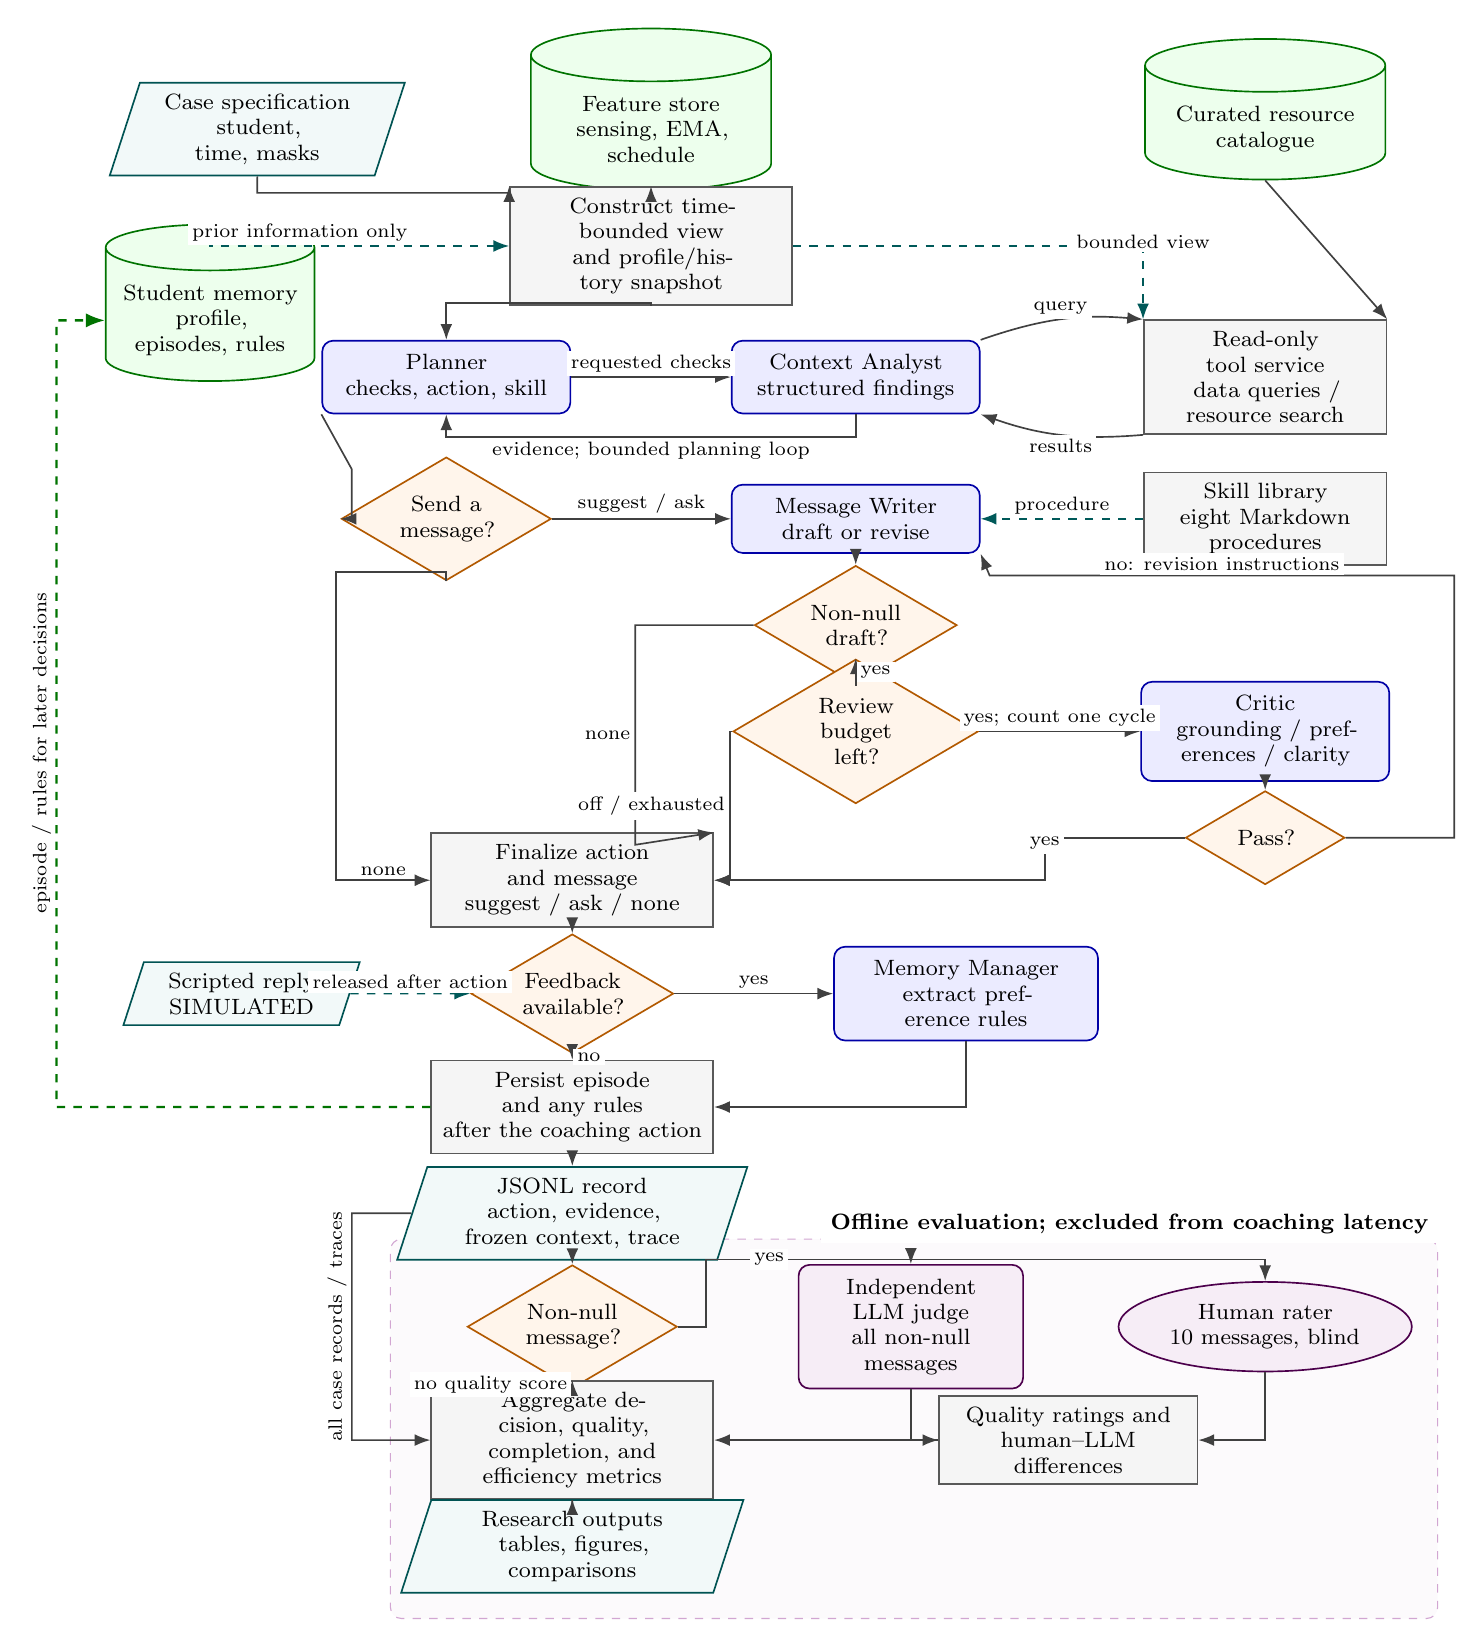
\begin{tikzpicture}[x=1cm,y=.90cm,
  font=\fontsize{8.2}{9.2}\selectfont,
  >=Latex, line width=.6pt,
  agent/.style={rounded corners=4pt,draw=blue!65!black,fill=blue!8,
      minimum height=.75cm,text width=2.8cm,align=center,inner sep=5pt},
  proc/.style={rectangle,draw=black!65,fill=black!4,minimum height=.7cm,
      text width=3.3cm,align=center,inner sep=4pt},
  io/.style={trapezium,trapezium left angle=72,trapezium right angle=108,
      draw=teal!65!black,fill=teal!5,minimum height=.75cm,text width=2.7cm,align=center,inner sep=4pt},
  db/.style={cylinder,shape border rotate=90,aspect=.22,draw=green!45!black,
      fill=green!7,minimum height=.9cm,text width=2.7cm,align=center,inner sep=5pt},
  gate/.style={diamond,aspect=1.7,draw=orange!70!black,fill=orange!8,
      text width=1.5cm,align=center,inner sep=1pt},
  edge/.style={->,draw=black!75},
  context/.style={->,dashed,draw=teal!70!black},
  write/.style={->,dashed,draw=green!45!black,line width=.85pt},
  lab/.style={fill=white,inner sep=1.5pt,font=\fontsize{7.5}{8.5}\selectfont}]

\node[io] (input) at (2,0) {Case specification\\student, time, masks};
\node[db] (features) at (7,0) {Feature store\\sensing, EMA, schedule};
\node[db] (resources) at (14.8,0) {Curated resource\\catalogue};
\node[proc] (context) at (7,-1.65) {Construct time-bounded view\\and profile/history snapshot};
\node[db,text width=2.3cm] (memory) at (1.4,-2.7) {Student memory\\profile, episodes, rules};
\node[agent] (planner) at (4.4,-3.5) {Planner\\checks, action, skill};
\node[agent] (analyst) at (9.6,-3.5) {Context Analyst\\structured findings};
\node[proc,text width=2.8cm] (tools) at (14.8,-3.5) {Read-only tool service\\data queries / resource search};
\node[gate] (action) at (4.4,-5.5) {Send a\\message?};
\node[agent] (writer) at (9.6,-5.5) {Message Writer\\draft or revise};
\node[proc,text width=2.8cm] (skills) at (14.8,-5.5) {Skill library\\eight Markdown procedures};
\node[gate] (message) at (9.6,-7.0) {Non-null\\draft?};
\node[gate] (review) at (9.6,-8.5) {Review\\budget left?};
\node[agent] (critic) at (14.8,-8.5) {Critic\\grounding / preferences / clarity};
\node[gate] (pass) at (14.8,-10.0) {Pass?};
\node[proc] (final) at (6,-10.6) {Finalize action and message\\suggest / ask / none};
\node[io,text width=2.2cm] (feedback) at (1.8,-12.2) {Scripted reply\\SIMULATED};
\node[gate] (reply) at (6,-12.2) {Feedback\\available?};
\node[agent,text width=3.0cm] (manager) at (11,-12.2) {Memory Manager\\extract preference rules};
\node[proc] (persist) at (6,-13.8) {Persist episode and any rules\\after the coaching action};
\node[io,text width=3.4cm] (output) at (6,-15.3) {JSONL record\\action, evidence, frozen context, trace};
\node[gate] (nonnull) at (6,-16.9) {Non-null\\message?};
\node[agent,text width=2.5cm,fill=violet!7,draw=violet!60!black] (judge) at (10.3,-16.9) {Independent LLM judge\\all non-null messages};
\node[ellipse,draw=violet!60!black,fill=violet!7,text width=2.4cm,align=center,minimum height=.8cm] (human) at (14.8,-16.9) {Human rater\\10 messages, blind};
\node[proc,text width=3.0cm] (ratings) at (12.3,-18.5) {Quality ratings and\\human--LLM differences};
\node[proc] (metrics) at (6,-18.5) {Aggregate decision, quality,\\completion, and efficiency metrics};
\node[io,text width=3.3cm] (results) at (6,-20.0) {Research outputs\\tables, figures, comparisons};

\draw[edge] (input.south) -- (2,-.9) -| (context.north west);
\draw[edge] (features) -- (context);
\draw[context] (memory.north) |- node[lab,pos=.65,above]{prior information only} (context.west);
\draw[edge] (context.south) -- (7,-2.45) -| (planner.north);
\draw[context] (context.east) -- (12.7,-1.65) -| node[lab,pos=.55,above]{bounded view} (tools.north west);
\draw[edge] (resources.south) -- (tools.north east);
\draw[edge] (planner.east) -- node[lab,above]{requested checks} (analyst.west);
\draw[edge] (analyst.south) -- (9.6,-4.35) -- node[lab,below]{evidence; bounded planning loop} (4.4,-4.35) -- (planner.south);
\draw[edge] (analyst.north east) to[bend left=12] node[lab,above]{query} (tools.north west);
\draw[edge] (tools.south west) to[bend left=12] node[lab,below]{results} (analyst.south east);
\draw[edge] (planner.south west) -- (3.2,-4.8) |- (action.west);
\draw[edge] (action.east) -- node[lab,above]{suggest / ask} (writer.west);
\draw[edge] (action.south) -- (4.4,-6.25) -- (3,-6.25) -- (3,-10.6) -- node[lab,above]{none} (final.west);
\draw[context] (skills.west) -- node[lab,above]{procedure} (writer.east);
\draw[edge] (writer) -- (message);
\draw[edge] (message) -- node[lab,right]{yes} (review);
\draw[edge] (message.west) -- (6.8,-7) -- node[lab,left]{none} (6.8,-10.1) -- (final.north east);
\draw[edge] (review.west) -- (8,-8.5) -- node[lab,left]{off / exhausted} (8,-10.6) -- (final.east);
\draw[edge] (review.east) -- node[lab,above]{yes; count one cycle} (critic.west);
\draw[edge] (critic) -- (pass);
\draw[edge] (pass.west) -- (12,-10) |- node[lab,pos=.2,above]{yes} (final.east);
\draw[edge] (pass.east) -- (17.2,-10) -- (17.2,-6.3) -- node[lab,above]{no: revision instructions} (11.3,-6.3) -- (writer.south east);
\draw[edge] (final) -- (reply);
\draw[context] (feedback) -- node[lab,above]{released after action} (reply);
\draw[edge] (reply.east) -- node[lab,above]{yes} (manager.west);
\draw[edge] (manager.south) |- (persist.east);
\draw[edge] (reply) -- node[lab,right]{no} (persist);
\draw[write] (persist.west) -- (-.55,-13.8) -- node[lab,rotate=90,above,pos=.45]{episode / rules for later decisions} (-.55,-2.7) -- (memory.west);
\draw[edge] (persist) -- (output);
\draw[edge] (output.west) -- (3.2,-15.3) -- node[lab,rotate=90,above]{all case records / traces} (3.2,-18.5) -- (metrics.west);
\draw[edge] (output) -- (nonnull);
\draw[edge] (nonnull.east) -- (7.7,-16.9) -- (7.7,-15.95) -- (14.8,-15.95) -- (human.north);
\draw[edge] (10.3,-15.95) -- (judge.north);
\node[lab] at (8.5,-15.95) {yes};
\draw[edge] (nonnull) -- node[lab,left]{no quality score} (metrics);
\draw[edge] (judge.south) |- (ratings.west);
\draw[edge] (human.south) |- (ratings.east);
\draw[edge] (ratings.west) -- (metrics.east);
\draw[edge] (metrics) -- (results);
\begin{scope}[on background layer]
  \node[draw=violet!35,dashed,fill=violet!2,rounded corners=4pt,
    fit=(nonnull)(judge)(human)(ratings)(metrics)(results),inner sep=9pt] (evalpanel) {};
\end{scope}
\node[font=\bfseries\fontsize{8.2}{9.2}\selectfont,anchor=east,fill=white] at (17,-15.45) {Offline evaluation; excluded from coaching latency};
\end{tikzpicture}
}
\caption{End-to-end workflow for the full five-role condition; alternatives are defined in Table~\ref{tab:controls}. Rounded blue boxes denote LLM coaching agents; gray rectangles deterministic processing; diamonds control decisions; cylinders persistent stores; parallelograms inputs/outputs; and the ellipse a human rater. Teal dashed links supply external context or procedures; the green dashed link updates memory for later decisions. Planning and review have explicit maximum budgets. A revised message can be finalized when the review budget is exhausted, so approval of the last draft is not guaranteed. Offline judging receives saved context and is excluded from coaching latency.}
\label{fig:workflow}
\end{figure*}

\begin{table*}[t]
\caption{Agent interfaces and execution conditions. The independent evaluator is outside the five-role coaching system.}
\label{tab:agents}\centering\small\setlength{\tabcolsep}{4pt}
\begin{tabular}{p{2.0cm}p{4.5cm}p{5.8cm}p{3.3cm}}\toprule
Role & Principal inputs & Structured outputs & Execution condition\\\midrule
Planner & Time context; profile/history; skill index; earlier plans and analyst reports & \code{status} (gather/finalize), hypotheses, checks, decision, skill, target goal, writer guidance, rationale & Planning enabled; within maximum planner-call budget\\
Context Analyst & Student/time; requested checks and hypotheses, or autonomous evidence policy; bounded tool closures & Findings with source/simulation tags; missing modalities; stress assessment; summary & At least one evidence pass in multi-agent mode; further passes when requested\\
Message Writer & Analyst reports; profile/history; plan and guidance when present; selected skill or skill index; optional draft and critique & Action, skill identifier, final message, rationale & Planner did not choose silence; can select action itself without planning\\
Critic & Draft, analyst reports, plan, profile/history, review index & Pass/revise verdict, critique, revision instructions & Non-null draft, reflection enabled, review budget remains\\
Memory Manager & Finalized action/message and explicitly simulated current reply & One to three actionable preference rules & Memory enabled and nonempty feedback text supplied\\\bottomrule
\end{tabular}
\end{table*}

\subsection{Bounded Planning and Evidence Gathering}
The Planner proposes checks, receives structured findings, and selects an action and a skill. A planning round is one Planner invocation. With a maximum of two or more rounds, the first call is instructed to request evidence, the Analyst executes checks, and a later Planner call can review that evidence. At least one Analyst pass executes; a finalize response can terminate planning early. Further information gathering is permitted only while the budget remains. At a maximum of one round, the Analyst first gathers evidence autonomously and the single Planner call then reviews it. This avoids requiring the one-round condition to decide without observations.

The Analyst obtains data through read-only Python callables bound to a student-specific temporal view. It receives requested checks and hypotheses rather than unrestricted dataset files. Findings identify sources and missing modalities. Disabling planning leaves the Analyst's evidence collection and the Writer's decision/skill selection active. A plan is therefore an explicit information-gathering and decision structure, rather than an unobserved claim about the model's internal reasoning.

\subsection{Tool Catalogue and Access}
Table~\ref{tab:tools} lists all eight data/resource tools. Recent windows default to three days, are clamped to 1--30 days, and use the availability boundaries in Section~\ref{sec:task}; deadline lookahead is clamped to 1--14 days. Resource search uses a small local catalogue, not web browsing. It ranks keyword matches, returns relevant descriptions and contacts, and uses a mental-health-category fallback when no keyword matches. These entries are curated demonstration content outside StudentLife, not recorded participant data or continuously verified historical service information.

\begin{table*}[t]
\caption{Data/resource tools available to the Context Analyst and consolidated coach. Missing or masked inputs return explicit status/reason fields rather than invented observations.}
\label{tab:tools}\centering\small\setlength{\tabcolsep}{4pt}
\begin{tabular}{p{5.0cm}p{3.1cm}p{7.5cm}}\toprule
Callable & Arguments & Returned information\\\midrule
\tool{get_time_context} & None & Date, weekday, local time, time of day, term week/phase, current scheduled class when available.\\
\tool{get_sleep_summary} & \code{days=3} & Inferred and self-reported sleep, observation counts, available last-night estimate, bed/wake times, difference from prior baseline.\\
\tool{get_activity_summary} & \code{days=3} & Active, walk, and run minutes; days with coverage; baseline comparison; self-reported exercise.\\
\tool{get_social_summary} & \code{days=3} & Conversation count/duration, available calls/SMS and self-reported contact categories; missing conversation status and baseline.\\
\tool{get_stress_mood_history} & \code{days=3} & Stress mean/max/latest and recency, mood/PAM summaries, latest comment within 14 days, pre-term background scores.\\
\tool{get_academic_load} & \code{days_ahead=3} & Deadlines today and by upcoming day, today's class periods, remaining classes, course count, partial-schedule indicators.\\
\tool{compare_to_baseline} & \code{feature}, \code{days=3} & Recent mean, historical mean/SD and sample size, standardized difference, qualitative deviation label. Supports sleep, bedtime, activity, conversation, calls/SMS, stress, mood, and self-report sleep.\\
\tool{search_campus_resources} & \code{need} & Ranked curated resources: names, categories, descriptions, contacts, and provenance tag; up to three keyword-matched entries.\\\bottomrule
\end{tabular}
\end{table*}

There are also two auxiliary access tools. \tool{load_skill(name)} returns a skill's metadata, procedure, constraints, and examples. The Writer can invoke it when no full skill has been supplied or when revising; the consolidated coach also has access. \tool{recall_memory(query)} exposes the current permitted profile, rules, and history to the consolidated coach. The query is a topic label; retrieval is a bounded snapshot, not semantic vector search. The multi-agent workflow normally injects memory text directly into planning, writing, and criticism. Consequently, the Analyst is not the only role capable of tool use.

\subsection{Skill-Guided Message Generation}
A skill is a reusable Markdown procedure with a name, description, applicability conditions, contraindications, constraints, and examples. It changes the Writer's instructions; it does not invoke a separately trained model. The Planner usually selects a skill from its index and the orchestrator supplies the full document. Without a Planner, the Writer chooses a skill and can load it through the auxiliary tool. Table~\ref{tab:skills} gives the complete library.

\begin{table*}[t]
\caption{The eight reusable coaching skills. Applicability statements are prompt-level guidance, not a deterministic guarantee that every output satisfies a constraint.}
\label{tab:skills}\centering\small\setlength{\tabcolsep}{4pt}
\begin{tabular}{p{4.6cm}p{5.4cm}p{5.6cm}}\toprule
Skill identifier & Intended use and procedure & Principal constraints\\\midrule
\tool{micro_study_break} & Elevated load/stress: acknowledge context and offer a short screen-free, breathing, stretching, or refreshment break. & Respect class/sleep context, quiet settings, preferences, and stricter length limits; avoid a long checklist.\\
\tool{sleep_hygiene_nudge} & Short or irregular sleep: connect evidence to upcoming demands and suggest one manageable wind-down cue. & Supportive, non-diagnostic language; no rigid universal sleep prescription; usually under 65 words.\\
\tool{gentle_movement} & Activity below baseline or suitable stress context: offer a short low-intensity walk or indoor stretch. & Respect rejected exercise types and setting; prefer indoor options late in the evening.\\
\tool{social_reconnection} & Reduced contact or relevant loneliness background: offer an optional, low-pressure connection. & No shaming; avoid social/group suggestions when prior preferences request solo recovery; concise wording.\\
\tool{deadline_chunking} & Imminent/clustered deadlines: name the known load and propose one small time-boxed next step. & Do not invent assignment names; preserve autonomy, preferred break style, and length constraints.\\
\tool{campus_resource_referral} & Distress or relevant support need: acknowledge the situation and surface a suitable curated resource with an optional small immediate step. & No diagnosis; resource details must come from the catalogue or supplied skill content; avoid unnecessary escalation for a comfortable student.\\
\tool{clarifying_question} & Insufficient key modalities: acknowledge missing information and ask one easy question. & No fabrication from background surveys; one low-burden question, brief wording (target under 45 words).\\
\tool{positive_reinforcement} & Stable or improved patterns when a message is warranted: acknowledge a concrete positive behavior. & Prefer silence on calm days or after an accepted message; do not invent problems; keep any acknowledgment under 40 words.\\\bottomrule
\end{tabular}
\end{table*}

\subsection{Critique, Revision, and Action Consistency}
The Writer emits a structured action, skill, and message. When planning is active, its first draft follows the Planner's action. The Critic checks factual grounding, available evidence, goal alignment, baseline and learned constraints, clarity, and appropriateness. A pass ends review; a revise verdict supplies instructions to another Writer call. Revisions can change the final action or selected skill, and the serialized output uses the current Writer result.

One reflection cycle is one Critic review and, if requested, its associated revision. A maximum of two cycles does not force two reviews: approval stops the loop. If the last permitted review requests revision, the Writer can revise once more and the result is emitted without an additional review beyond the budget. A revised silence decision also stops the loop. Reflection is thus a bounded quality-control mechanism, not a guarantee of factual or clinical correctness.

\subsection{Longitudinal Memory and Feedback}
For each student, persistent JSON stores \code{profile}, \code{episodes}, and \code{learned_preferences}. An episode includes its case identifier, decision time, action, selected skill, message, and simulated reply. A learned rule includes its text, source case, timestamp, and simulation label. Baseline goals/preferences remain separate from rules extracted from later feedback; repeated identical rule strings are deduplicated.

At time $t$, the memory snapshot includes only episodes and rules with timestamps strictly less than $t$. Up to five recent episodes are placed in prompts, while eligible learned rules can persist beyond that episode window. Feedback stamped with the current case is excluded from that case's decision and becomes usable at a later time. Each participant's cases run in chronological order across episode identifiers; different participants can run concurrently. Read-modify-write operations are protected so an update records the episode and its rules together.

The Memory Manager is called only when memory is enabled and a nonempty scripted reply exists. It extracts one to three actionable rules after finalizing the message. This is a language-model-mediated update over a file store; no SQLite database, knowledge graph, embedding index, or live student chat is involved. The present evaluation does not establish robust conflict resolution for contradictory long-term feedback.

\subsection{Configuration and Final System}
Table~\ref{tab:controls} connects each required design pattern to an explicit control and its operational meaning. The final full configuration retains all five coaching roles and all five patterns, with planning/review maxima of two, memory history length five, and the eight-skill library. This is a system-design choice evaluated against alternatives, not a claim that every enabled component improves every measured outcome.

\begin{table*}[t]
\caption{Pattern controls in multi-agent mode and the final settings. The single-coach mode consolidates online reasoning roles and bypasses the separate Planner and Critic loops.}
\label{tab:controls}\centering\small\setlength{\tabcolsep}{4pt}
\begin{tabular}{p{2.1cm}p{4.7cm}p{6.8cm}p{2.0cm}}\toprule
Pattern & Configuration & Meaning of disabling/varying & Full setting\\\midrule
Multi-agent & \code{system.mode} & \code{single_agent} consolidates retrieval, action/skill selection, and writing into one online coach; shared feedback extraction remains auxiliary. & Five coaching roles\\
Planning & \code{planning.enabled}, \code{max_rounds} & Off: autonomous Analyst then Writer selects action/skill. Maxima 1, 2, 3 bound actual Planner calls. & On; maximum 2\\
Tool use & \code{tools.enabled}, \code{max_turns} & Off: multi-agent Analyst receives a fixed evidence summary instead of choosing data queries. Tool-selection autonomy is removed, not all data. & On; 5 tool-loop turns\\
Reflection & \code{reflection.enabled}, \code{max_rounds} & Off: omit Critic. Maxima 1, 2, 3 limit review/revision cycles with early approval. & On; maximum 2\\
Memory & \code{memory.enabled}, \code{history_k} & Off: omit earlier episodes/rules from prompts and skip preference extraction; retain the baseline profile. Episode logging may still occur. & On; 5 recent episodes\\
Skills & \code{skills.enabled} & Off: omit skill index/documents and skill-loading access; use general supportive instructions. & On; 8 procedures\\\bottomrule
\end{tabular}
\end{table*}

\subsection{Worked Interaction: From Evidence to Memory}\label{sec:example}
Consider student \code{u16} on April 18 at 20:00 (\code{case_014}). Available three-day context includes one deadline that day, mean stress 3.3/5 with maximum 4/5, and one inferred sleep observation averaging 6.5 hours. The simulated baseline profile favors gentle, concise, quiet indoor breaks. Feedback from April 15 has already supplied rules rejecting running/gym suggestions during deadlines and preferring indoor stretching, breathing, or tea.

The Planner requests evidence; the Analyst supplies source-tagged observations. A second Planner call selects \code{suggest} and \code{micro_study_break}. The Writer produces:
\begin{quote}\smallWith today's deadline and midterm week in full swing, you've been working hard through a stressful day. If you need a quick reset tonight, pause for 5 minutes to take a few slow, deep breaths or pour a warm cup of tea before diving back in.\end{quote}
The Critic passes the draft after one review. The record reports two Planner calls, seven completed LLM calls overall, five tool calls, 18,146 tokens, and 55.54 seconds of end-to-end case latency. The seven LLM calls include subsequent preference extraction, rather than representing seven different agents.

Only after this message is finalized does the scripted reply add a library-compatible, under-35-word preference. The Memory Manager stores it for later decisions. On April 22, the same student's final message is:
\begin{quote}\smallMidterms and today's deadline can feel overwhelming. Take a quick 5-minute quiet pause right at your desk to sip warm tea and do a few slow, deep breaths.\end{quote}
This example illustrates temporal use of feedback: the new length constraint applies to the later interaction, not retroactively to the April 18 message. Since the baseline profile already favors quiet breaks, the example demonstrates use of supplied preferences rather than proving an independent causal memory benefit. Appendix~\ref{app:io} gives structured input/output projections; Appendix~\ref{app:algorithm} specifies the control flow.

\section{Experimental Design}\label{sec:experiments}
\subsection{Cases and Selection}
We use 20 reproducible participant/time cases from \code{u59}, \code{u08}, \code{u19}, \code{u10}, \code{u57}, \code{u16}, \code{u00}, and \code{u02}. Selection emphasizes coverage of EMA stress and usable sensing, supplemented by low-stress and absent-observation windows. It is scenario-based selection rather than random sampling. The cases contain five high-stress/load situations, three doing-fine situations, four missing-data situations, six steps in two three-step preference episodes, and two support/restraint situations. All decisions are at 20:00 local time. Appendix~\ref{app:cases} lists the full manifest and masks.

Allowed actions are manually specified sets, not measured student responses. Most are single labels; one high-stress case allows either a suggestion or silence, and one absent-observation case permits a question or suggestion. This accommodates judgment under uncertain context, but it also makes allowed-label agreement a project-authored benchmark proxy. Expected actions and case-selection rationales are not supplied to coaching agents or evaluators.

\subsection{Models and Inference Settings}
Table~\ref{tab:models} identifies every LLM used. Model A supports function calling and structured responses for all coaching roles. Model B provides a lower-cost alternative under the same full architecture. A separate OpenAI judge avoids using either Gemini coaching model as its own message evaluator. These are design rationales; task suitability is assessed through the reported cases rather than assumed from a model's product label or provider.

\begin{table*}[t]
\caption{LLMs and generation settings. There is no training or fine-tuning. Critic and Memory Manager temperatures are 0.1; other coaching calls use 0.3.}
\label{tab:models}\centering\small\setlength{\tabcolsep}{4pt}
\begin{tabular}{p{2.3cm}p{6.4cm}p{3.2cm}p{3.7cm}}\toprule
Use & Provider and exact model identifier & Reasoning setting & Output and role settings\\\midrule
Model A & Google: \code{gemini-3.6-flash} & \code{thinking_level}\newline\code{low} & 8,192-token cap; all full-system and structural-ablation coaching roles\\
Model B & Google: \code{gemini-3.5-flash-lite} & \code{thinking_level}\newline\code{low} & Same temperature/cap and full architecture as Model A\\
Independent judge & OpenAI: \code{gpt-5.4-mini-2026-03-17} & \code{reasoning_effort}\newline\code{none} & Temperature 0; 2,048 completion-token cap; structured integer ratings\\\bottomrule
\end{tabular}
\end{table*}

The multi-agent tool-assisted Analyst/Writer interactions permit up to five model turns per tool loop. The consolidated coach permits seven to accommodate its combined responsibilities. Multiple Python functions can be called within a turn; a turn limit is not an identical limit on Python calls. Four workers process independent participant histories, with one-second provider-request spacing per credential. Requests retain the condition's model during retry. These allocations and remote service conditions mean the comparison is not a compute-matched benchmark.

\subsection{Required Ablation Conditions}
The full condition is compared with eight alternatives: (1) one consolidated online coach, (2) no Critic/reflection, (3) no Planner, (4--5) reflection maxima of one and three, (6--7) planning maxima of one and three, and (8) Model B with the full settings. Full supplies the maximum-two reference for both depth studies, so nine conditions cover all six comparison types.

The consolidated baseline receives the same exogenous observations, baseline profile, scenario scripts, available data tools, skills, and history-retrieval policy. It combines online analysis, action/skill selection, and writing in one role. The shared post-feedback Memory Manager remains auxiliary in both conditions; ``single coach'' therefore describes the online decision maker, not an assertion that every LLM-assisted maintenance operation has disappeared. Separate role-based planning/reflection budgets are bypassed there.

Each condition has its own memory state. Because earlier messages and extracted rules can differ, later history contents can diverge between conditions even with identical initial inputs and feedback scripts. We interpret the results as longitudinal workflow comparisons, not strictly identical-history, single-prompt causal effects. No separate tool-, skill-, or memory-removal experiments are claimed; those modules are configurable, while the conducted comparisons follow the six specified types.

\subsection{Independent Message Evaluation}\label{sec:judging}
All successful non-null messages receive integer 1--5 ratings for context awareness, goal alignment, and clarity. The judge also returns a Boolean indicating whether sending the message was appropriate and a concise justification. Silence receives no fictitious quality score; its action is evaluated through the allowed-action check. The exact anchored rubric is reproduced in Appendix~\ref{app:rubric}.

Human and automated evaluators receive the same saved packet: a deterministic evidence summary; baseline profile; learned rules; earlier episodes; any simulated recent-interaction note; and the final action, skill, and message. The summary includes three-day sleep/activity/social/academic summaries, three- and seven-day stress summaries, and seven-day baseline comparisons. It is assembled at the decision time, before the current feedback update.

This packet is not a verbatim copy of every agent prompt or queried tool response. An Analyst may use other windows or resource-search results, and a Writer may see a full skill procedure that is absent from the evaluator packet. Thus identical human--LLM evaluator context is established, while complete equality with all dynamically gathered coaching context is not. This limits the evaluator's ability to verify every resource detail or agent-specific observation.

One human rater, Mahdi Moghaddami, independently scores 10 full-system messages using the same rubric before viewing the automated judge's scores. Items follow a fixed scenario-based priority, skipping null messages; they are not selected by judge score. There is one rater and no inter-rater reliability estimate. The 140 non-null messages across conditions are judged independently of the human scores.

\subsection{Metrics and Measurement Boundaries}\label{sec:metrics}
For $N$ cases with allowed-action sets $A_i$, action agreement is
\begin{equation}
\mathrm{Agree}=\frac{1}{N}\sum_i\mathbb{1}[\mathrm{success}_i\land a_i\in A_i].
\end{equation}
Completion is the fraction with a valid successful final record, after permitted retries. Failed records are reported separately and do not count as successful silence. For the $N_m$ scored messages and three criteria $q_{ik}$,
\begin{equation}
Q=\frac{1}{3N_m}\sum_{i=1}^{N_m}\sum_{k=1}^{3}q_{ik}.
\end{equation}
Because conditions can send different numbers of messages, we additionally compare quality on the intersection of non-null case IDs shared with full. Judge sending-appropriateness is a separate percentage over non-null messages; it is not the same as allowed-label agreement over all cases.

For $n=10$ paired human and judge messages,
\begin{align}
\mathrm{MAD}_{\mathrm{criterion}}&=\frac{1}{3n}\sum_{i,k}|h_{ik}-q_{ik}|,\\
\mathrm{MAD}_{\mathrm{message}}&=\frac{1}{n}\sum_i|\overline h_i-\overline q_i|.
\end{align}
The second measure can be smaller because opposing criterion differences cancel before the absolute value is taken.

Preference adherence is a deterministic proxy on four later steps in the two feedback episodes. It checks forbidden terms, at least one required theme from each applicable earlier feedback step, and the latest supplied word limit. The current reply is excluded. This lexical check is supplementary to semantic goal-alignment ratings and can produce false positives.

Latency spans case start to valid final output, including data access, tools, model steps, memory updates, provider waits, and any re-execution needed for a valid chronological history; offline judging is excluded. Calls/tokens in case traces count recorded completed model steps. Successful provider responses inside an attempt that later fails may consume additional tokens, so provider-level ledgers supply complementary totals. For dependent re-executions, derived efficiency adds recorded work across attempts and includes elapsed scheduling time. These definitions avoid equating a successful final trace with cost-free request failures.

\FloatBarrier
\section{Results}\label{sec:results}
\subsection{Full-System Behavior}
The full system produces 20 valid records, matches all 20 allowed-action sets, and sends 16 messages: 13 suggestions and three questions. Four cases yield silence. Mean message quality is 4.81/5; context awareness is 4.75, goal alignment 4.94, and clarity 4.75. The independent judge considers sending each of the 16 messages appropriate. Table~\ref{tab:categories} shows scenario coverage and quality without assigning scores to silence.

\begin{table}[t]
\caption{Full-system scenario results. $N_m$ counts non-null messages. ``Agreement'' means membership in the manually allowed action set.}
\label{tab:categories}\centering\scriptsize\setlength{\tabcolsep}{3pt}
\resizebox{\columnwidth}{!}{\begin{tabular}{lrrrr}
\toprule
Scenario & $N$ & $N_m$ & Agreement (\%) & Quality \\
\midrule
High stress/load & 5 & 5 & 100 & 4.60 \\
Doing fine & 3 & 0 & 100 & --- \\
Missing data & 4 & 4 & 100 & 5.00 \\
Preference episodes & 6 & 6 & 100 & 4.94 \\
Support/restraint & 2 & 1 & 100 & 4.33 \\
\bottomrule
\end{tabular}
}
\end{table}

These results support successful execution on the selected cases and illustrate suggestions, uncertainty-aware questions, and restraint. They do not establish perfect intervention decisions outside the benchmark. The worked example in Section~\ref{sec:example} also shows use of previous feedback; four designated later preference steps pass the full system's lexical checks, a small measure of consistency rather than evidence of broad longitudinal effectiveness.

\subsection{Human--LLM Agreement}
Table~\ref{tab:human} reports results on the same 10 messages. Human means are 4.70 for context, 4.80 for goals, and 5.00 for clarity. The corresponding judge means are 4.80, 4.90, and 4.60. Criterion-level MAD is 0.267 across 30 scores; per-message-average MAD is 0.133. These are different summaries, not conflicting estimates of the same calculation.

\begin{table*}[t]
\caption{Independent human and LLM ratings on 10 identical full-system messages. Means are shown with sample standard deviations. MAD is defined in Section~\ref{sec:metrics}; the final row first averages criteria within each message.}
\label{tab:human}\centering\small\begin{tabular}{lrrrr}
\toprule
Criterion & Human & LLM judge & MAD & LLM $-$ human \\
\midrule
Context awareness & $4.70\pm0.67$ & $4.80\pm0.42$ & 0.100 & +0.100 \\
Goal alignment & $4.80\pm0.42$ & $4.90\pm0.32$ & 0.300 & +0.100 \\
Clarity & $5.00\pm0.00$ & $4.60\pm0.70$ & 0.400 & -0.400 \\
Per-message average & $4.83\pm0.28$ & $4.77\pm0.45$ & 0.133 & -0.067 \\
\bottomrule
\end{tabular}

\end{table*}

The largest discrepancy is \code{case_002}: human clarity is 5 and judge clarity is 3. The judge describes the bedtime suggestion as wordy and more certain than necessary; the human supplied no explanatory note, so we do not infer their reasoning. The same message also differs by one point in context and goal alignment. Other one-point differences show that a warm, understandable message can still be judged differently for concision or preference fit. High scores and a single author-rater also create ceiling effects and limit claims of calibrated agreement.

\subsection{Architecture, Planning, and Reflection Ablations}
Table~\ref{tab:quality} presents all required conditions. Each condition has 20 valid final records. Initial-attempt completion is 95\% for planning maximum three and 100\% for the others; the table reports successful final completion after retry. Final completion should therefore be read alongside latency and provider-failure accounting, not as a claim that no request ever failed.

\begin{table*}[t]
\caption{Nine conditions on identical case definitions. $N_m$ is the scored-message count. Agreement uses allowed actions over all 20 cases; Send OK is the independent judge's appropriateness percentage over non-null messages. Quality criteria are scored 1--5.}
\label{tab:quality}\centering\small\setlength{\tabcolsep}{4pt}
\resizebox{\textwidth}{!}{\begin{tabular}{lrrrrrrrr}
\toprule
Condition & Completion (\%) & Agreement (\%) & $N_m$ & Context & Goal & Clarity & Mean & Send OK (\%) \\
\midrule
Full & 100 & 100 & 16 & 4.75 & 4.94 & 4.75 & 4.81 & 100.00 \\
Single coach & 100 & 100 & 16 & 4.88 & 4.88 & 4.69 & 4.81 & 100.00 \\
No planning & 100 & 100 & 16 & 4.69 & 4.75 & 4.69 & 4.71 & 100.00 \\
Planning max. 1 & 100 & 95 & 15 & 4.73 & 4.80 & 4.80 & 4.78 & 100.00 \\
Planning max. 3 & 100 & 95 & 15 & 4.87 & 4.87 & 4.87 & 4.87 & 100.00 \\
No reflection & 100 & 90 & 15 & 4.67 & 4.93 & 4.73 & 4.78 & 100.00 \\
Reflection max. 1 & 100 & 100 & 16 & 4.50 & 4.69 & 4.69 & 4.63 & 93.75 \\
Reflection max. 3 & 100 & 100 & 16 & 4.75 & 4.94 & 4.81 & 4.83 & 100.00 \\
Model B & 100 & 95 & 15 & 4.93 & 4.93 & 4.80 & 4.89 & 100.00 \\
\bottomrule
\end{tabular}
}
\end{table*}

\paragraph{Role decomposition.} The consolidated coach matches the full system's rounded quality mean of 4.81 and 100\% allowed-label agreement. Its mean latency is 18.78 rather than 35.59 seconds, and it uses fewer recorded model calls (3.65 versus 6.20), but more trace tokens on average (18,681 versus 17,529). These observations do not establish a general quality advantage for five-role decomposition. They show that fewer role calls need not imply fewer input/output tokens.

\paragraph{Planning.} Removing planning retains 100\% allowed-label agreement but reduces overall mean quality to 4.71. Maximum-one and maximum-three planning each obtain 95\% agreement, with quality means 4.78 and 4.87. The maximum-three condition actually averages 2.05 Planner invocations, compared with two in full and one in the depth-one condition. Most cases therefore do not consume a third planning round. The depth-one condition also uses Analyst-first ordering, so its comparison changes the schedule as well as the Planner-call limit. The highest allowed budget is not consistently best for action agreement.

\paragraph{Reflection.} Removing the Critic yields 90\% allowed-label agreement and 4.78 mean quality. Maximum-one, full maximum-two, and maximum-three reflection obtain quality means 4.63, 4.81, and 4.83, all with 100\% allowed-label agreement. However, all three average exactly one executed Critic cycle per sent message. The larger maxima do not create deeper actual review trajectories in these observations; score differences cannot be confidently attributed to additional executed reflection. Stochastic generation, differing drafts, and downstream histories remain explanations.

\begin{figure*}[t]
\centering
\begin{minipage}{.49\textwidth}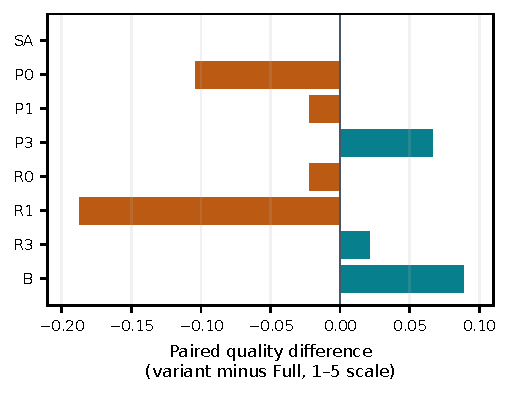
\includegraphics[width=\linewidth]{figures/paired_quality.pdf}\end{minipage}\hfill
\begin{minipage}{.49\textwidth}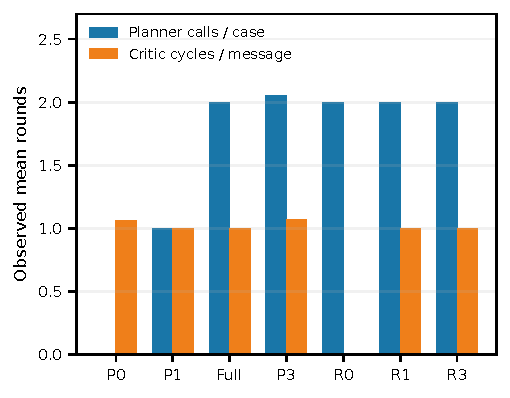
\includegraphics[width=\linewidth]{figures/effective_rounds.pdf}\end{minipage}
\caption{Left: variant-minus-full quality on common non-null case IDs. Right: actual Planner invocations and Critic cycles, showing that a configured maximum does not imply that all rounds execute. SA denotes the consolidated coach; P0/P1/P3 planning maxima 0/1/3; R0/R1/R3 reflection maxima 0/1/3; B Model B; Full uses maxima two for both. These single-run differences are descriptive.}
\label{fig:paired}
\end{figure*}

Table~\ref{tab:paired} and Figure~\ref{fig:paired} restrict quality comparisons to shared non-null cases. The single-coach difference is zero, no planning is $-0.104$, no reflection is $-0.022$, and Model B is $+0.089$ on this paired scale. Small differences over 15--16 messages do not establish statistical superiority, especially with repeated participant identities and no repeated-generation sampling.

\begin{table}[t]
\caption{Quality on the same non-null case IDs in full and each variant. Positive $\Delta$ favors the variant.}
\label{tab:paired}\centering\scriptsize\setlength{\tabcolsep}{3pt}
\begin{tabular}{lrrrr}
\toprule
Condition & $N_\cap$ & Full & Variant & $\Delta$ \\
\midrule
Single coach & 16 & 4.813 & 4.813 & +0.000 \\
No planning & 16 & 4.813 & 4.708 & -0.104 \\
Planning max. 1 & 15 & 4.800 & 4.778 & -0.022 \\
Planning max. 3 & 15 & 4.800 & 4.867 & +0.067 \\
No reflection & 15 & 4.800 & 4.778 & -0.022 \\
Reflection max. 1 & 16 & 4.813 & 4.625 & -0.188 \\
Reflection max. 3 & 16 & 4.813 & 4.833 & +0.021 \\
Model B & 15 & 4.800 & 4.889 & +0.089 \\
\bottomrule
\end{tabular}

\end{table}

\subsection{Model Choice and Efficiency}
Model B produces 15 messages, reaches 95\% allowed-action agreement, and obtains 4.89 mean quality. It averages 21.60 seconds and 14,356 trace tokens per case. The corresponding full Model A values are 35.59 seconds and 17,529 tokens. Its higher writing score alongside one fewer matched decision illustrates why message quality and action selection should be evaluated separately. The full configuration remains a five-role demonstration with all requested patterns, rather than a data-derived assertion that its model and every component dominate alternatives.

\begin{table*}[t]
\caption{Efficiency across all cases in each condition. Latency, LLM calls, and tokens are mean $\pm$ sample SD. Actual Planner calls are per case; Critic cycles are per non-null message. Elapsed latency includes provider waits and any dependent re-execution, while judging is excluded. Remote service variability limits causal speed comparisons.}
\label{tab:efficiency}\centering\small\setlength{\tabcolsep}{5pt}
\begin{tabular}{lrrrrr}
\toprule
Condition & Latency (s) & LLM calls & Tokens ($10^3$) & Planner calls & Critic cycles \\
\midrule
Full & $35.59\pm15.12$ & $6.20\pm1.15$ & $17.53\pm2.88$ & 2.00 & 1.00 \\
Single coach & $18.78\pm9.29$ & $3.65\pm0.67$ & $18.68\pm5.32$ & 0.00 & 0.00 \\
No planning & $49.63\pm27.02$ & $6.10\pm1.68$ & $18.37\pm5.89$ & 0.00 & 1.06 \\
Planning max. 1 & $46.27\pm34.10$ & $5.40\pm1.43$ & $15.30\pm3.78$ & 1.00 & 1.00 \\
Planning max. 3 & $80.79\pm106.10$ & $6.95\pm2.48$ & $20.37\pm7.31$ & 2.05 & 1.07 \\
No reflection & $68.54\pm87.14$ & $5.35\pm0.81$ & $15.98\pm2.11$ & 2.00 & 0.00 \\
Reflection max. 1 & $46.38\pm27.38$ & $6.25\pm1.21$ & $17.92\pm3.60$ & 2.00 & 1.00 \\
Reflection max. 3 & $52.94\pm37.15$ & $6.10\pm1.02$ & $17.35\pm2.88$ & 2.00 & 1.00 \\
Model B & $21.60\pm9.88$ & $5.80\pm1.28$ & $14.36\pm2.93$ & 1.95 & 1.00 \\
\bottomrule
\end{tabular}

\end{table*}

Table~\ref{tab:efficiency} and Figure~\ref{fig:efficiency} expose the latency variation. Full uses 6.20 recorded LLM calls per case and 17,529 mean trace tokens. Some alternatives with fewer planned steps have larger measured latency because service waits and repeated attempts are included. Across conditions, provider ledgers record 1,085 successful generation requests and 178 failed provider attempts; these are distinct from 180 final case records. Thus the latency numbers describe this execution environment, not isolated model compute time or a platform-independent speed ranking.

\begin{figure*}[t]
\centering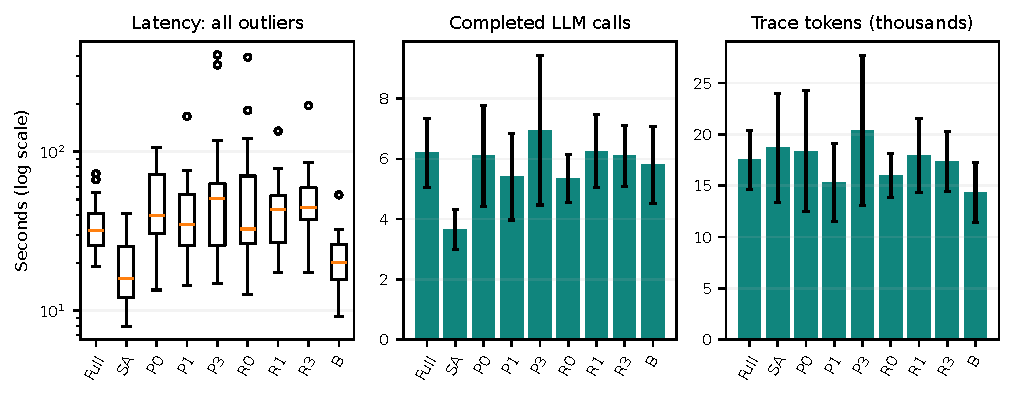
\includegraphics[width=\textwidth]{figures/efficiency.pdf}
\caption{Case-level efficiency, using the abbreviations in Figure~\ref{fig:paired}. The latency axis is logarithmic and includes all outliers. Calls and token bars include standard-deviation error bars. Recorded completed-step counts and provider-attempt accounting measure different aspects of execution.}
\label{fig:efficiency}
\end{figure*}

\subsection{Preference Measurement and Qualitative Inspection}
The full, no-planning, and depth variants pass all four designated lexical preference checks. The consolidated coach, no-reflection condition, and Model B each score 75\%. Inspection of the three flags indicates proxy false positives: ``stress running elevated'' and ``sleep running around 6.5 hours'' use \emph{running} without recommending exercise; Model B proposes ``a favorite song,'' which expresses music without matching a required keyword. We retain the literal proxy percentages and do not present these flags as demonstrated semantic preference failures. Appendix~\ref{app:preference} reports the counts and phrases. Inspecting flagged messages does not independently validate all unflagged messages.

\section{Discussion and Limitations}\label{sec:limitations}
The architecture makes agentic components observable: plans specify checks, tools return bounded evidence, skills supply procedures, the Critic returns a verdict, and memory retains previous suggestions and rules. This explicit structure supports inspection and configurable comparisons even when mean quality does not improve over a consolidated coach. The results favor a multi-metric interpretation: action restraint, message fit, and efficiency can move in different directions.

The study has several limitations. Twenty hand-selected cases from eight identifiers are not independent population samples, and some missing-data cases occur beyond passive recording coverage. Simulated goals and deterministic replies do not measure genuine acceptance or preference formation. The baseline profiles sometimes already express the preferences reiterated in feedback, weakening causal claims about learning. Pre-term psychological scores are background context; these experiments do not establish valid current-risk classifications from those scores.

Only one generation per condition and one human rater are available. No confidence interval over repeated model generations or participant-level generalization is estimated. Different conditions can carry different endogenous histories; the consolidated coach has a different tool-turn allocation and shares auxiliary memory extraction. These factors limit an interpretation as isolated, compute-matched causal effects of one component.

The human and LLM evaluators share a frozen summary, but it may omit agent-specific tool windows, resource details, and loaded skill text. The judge cannot fully verify material absent from its packet, and high scores do not remove known LLM-judge biases. Lexical preference checks have observable false positives. Remote-provider delays and re-execution affect latency and cannot be cleanly assigned to architectural depth.

Finally, inferred sleep and conversation measures are noisy proxies. Static campus resources are demonstration content and are not verified against every historical decision date. The experiment measures offline coaching behavior, not resource availability, clinical effectiveness, academic improvement, or a change in stress. These are empirical boundaries of the present task.

\section{Conclusion}
We present a configurable student stress coach that combines five language-agent roles with time-bounded evidence tools, eight reusable skills, and persistent feedback memory. The full system demonstrates the required patterns, produces all 20 final case records, and receives strong but non-perfect independent quality ratings. Human--judge differences are small on average while exposing disagreement about clarity. The ablations show that role decomposition and larger budgets are not uniformly beneficial, and that an alternative model's writing score can improve while action agreement decreases. Broader case selection, repeated generations, independent raters, fuller evaluator context, and semantic preference measures are needed to extend these descriptive results.

\renewcommand{\bibfont}{\small}
\setlength{\bibsep}{0pt}
\bibliography{references}
\bibliographystyle{icml2026}
\clearpage\appendix\onecolumn\raggedbottom

\section{Structured Inputs and Outputs}\label{app:io}
The case file identifies a student, timestamp, modality masks, scenario labels, and any held-out scripted reply. Runtime inputs materialize the appropriate feature view and memory snapshot. The following compact projection of \code{case_014} illustrates the observations and prior context; its prose goal/feedback summaries abbreviate the underlying simulated profile and history. It excludes the reply delivered after that decision.
\lstinputlisting{examples/input.json}

The corresponding output projection preserves actual decision, message, evidence entries, and measured trace values. It is formatted across lines for readability here; the saved experiment uses one JSON object per JSONL line. Complete \code{evaluation_context}, critique text, memory-update strings, and other metadata are omitted from this projection and defined below.
\lstinputlisting{examples/output.json}

\clearpage\small
\begin{longtable}{p{3.5cm}p{2.1cm}p{10.2cm}}
\caption{Complete final-record field definitions. Expected labels and scenario metadata support offline analysis and are not supplied as answers to agents.}\label{tab:schema}\\
\toprule Field & Type & Meaning\\\midrule\endfirsthead
\toprule Field & Type & Meaning\\\midrule\endhead
\code{case_id} & String & Unique participant/time evaluation identifier.\\
\code{participant_id} & String & Dataset identifier, such as \code{u16}.\\
\code{decision_time} & ISO timestamp & Localized decision time with UTC offset.\\
\code{category} & String & Offline scenario category.\\
\code{episode_id} & String & Longitudinal scenario grouping; chronological memory also spans groups for the same student.\\
\code{step} & Integer & Position in the declared scenario episode.\\
\code{config_id} & String & Experimental configuration identifier.\\
\code{model} & String & Configured provider/model identifier for generation.\\
\code{status} & String & Successful execution or a failed case; failure is not equivalent to deliberate silence.\\
\code{error} & String/null & Execution error description on failure.\\
\code{decision} & Enum & \code{suggest}, \code{ask}, or \code{none}.\\
\code{expected_decision} & String list & Manually allowed actions for offline agreement scoring.\\
\code{skill_used} & String/null & Skill identifier for a sent message; null for silence.\\
\code{plan} & String list & Collected explicit planning steps or baseline's stated checks.\\
\code{evidence} & Object list & Source-tagged factual findings, details, and simulation flags.\\
\code{evaluation_context} & Object & Saved summary, simulated profile, prior rules/interactions, and scenario note for evaluators; absent from a failed record that could not construct it.\\
\code{final_message} & String/null & Final supportive suggestion or clarification; null for \code{none}.\\
\code{reflection} & Object & Actual review count and collected critique/verdict text.\\
\code{planning} & Object & Number of actual Planner invocations.\\
\code{memory_updates} & String list & Newly recorded preference rules from post-action simulated feedback.\\
\code{trace} & Object & Recorded LLM/tool calls, prompt/completion/total tokens, latency, per-role usage, and model identifiers. Total tokens may include reasoning tokens beyond visible completion text.\\
\bottomrule
\end{longtable}\normalsize

\Needspace{9cm}
\section{Coaching Control Procedure}\label{app:algorithm}
\begin{algorithm}[H]\footnotesize
\caption{One student/time interaction (maximum planning $P$, review $R$)}
\begin{algorithmic}[1]
\REQUIRE Student $u$, time $t$, time-bounded observations, baseline profile, earlier memory; optional held-out reply $F_t$
\STATE Construct bounded data tools and retrieve only episodes/rules dated before $t$.
\STATE Save the deterministic evaluator context, excluding $F_t$ and expected labels.
\IF{consolidated-coach mode}
  \STATE One online role inspects tools, selects action/skill, and drafts the message.
\ELSE
  \STATE With planning off, collect autonomous Analyst evidence and skip Planner calls.
  \STATE With planning on and $P=1$, collect Analyst evidence before the one Planner call.
  \STATE With planning on and $P\geq2$, invoke Planner up to $P$ times; collect Analyst evidence at least once and whenever more checks are requested; stop at finalize.
  \STATE Skip writing only for a planned silence action; otherwise Writer drafts using evidence/memory and selects its own action/skill when no plan exists.
  \FOR{$r=1$ to $R$, while a non-null message exists and reflection is enabled}
    \STATE Critic returns pass or revision instructions.
    \IF{pass} \STATE Stop review. \ELSE \STATE Writer revises action, skill, and message. \ENDIF
  \ENDFOR
\ENDIF
\STATE Normalize silence to null message/skill; require a nonempty message for sent actions.
\IF{memory enabled and $F_t$ has feedback text} \STATE Memory Manager extracts actionable preference rules. \ENDIF
\STATE Persist this episode, $F_t$, and any rules for strictly later decisions.
\STATE Serialize final JSONL output, execution status, evidence, and measured trace.
\end{algorithmic}
\end{algorithm}

\section{Evaluation Case Manifest}\label{app:cases}
All timestamps below are at 20:00 in \texttt{America/New\_York}. Preference cases 013--015 and 016--018 are two separate three-step scripts. The synthetic masks in cases 011--012 are distinct from the post-recording absence in 009--010. An empty mask does not imply complete observed data.
\begin{center}\small\begin{tabular}{lllp{3.0cm}p{3.7cm}l}
\toprule
Case & Student & Date & Scenario & Synthetic Mask & Allowed Action(s) \\
\midrule
001 & u59 & 2013-04-29 & High stress/load & None & suggest \\
002 & u08 & 2013-04-21 & High stress/load & None & suggest \\
003 & u19 & 2013-04-30 & High stress/load & None & suggest \\
004 & u10 & 2013-04-07 & High stress/load & None & suggest / none \\
005 & u57 & 2013-04-30 & High stress/load & None & suggest \\
006 & u57 & 2013-03-28 & Doing fine & None & none \\
007 & u02 & 2013-04-01 & Doing fine & None & none \\
008 & u00 & 2013-05-17 & Doing fine & None & none \\
009 & u00 & 2013-06-10 & Missing data & None & ask \\
010 & u57 & 2013-06-06 & Missing data & None & ask / suggest \\
011 & u08 & 2013-04-12 & Missing data & sleep, activity, stress & ask \\
012 & u19 & 2013-04-16 & Missing data & sleep, conversation, stress & ask \\
013 & u16 & 2013-04-15 & Preference episodes & None & suggest \\
014 & u16 & 2013-04-18 & Preference episodes & None & suggest \\
015 & u16 & 2013-04-22 & Preference episodes & None & suggest \\
016 & u59 & 2013-04-12 & Preference episodes & None & suggest \\
017 & u59 & 2013-04-15 & Preference episodes & None & suggest \\
018 & u59 & 2013-04-18 & Preference episodes & None & suggest \\
019 & u19 & 2013-05-07 & Support/restraint & None & suggest \\
020 & u57 & 2013-03-31 & Support/restraint & None & none \\
\bottomrule
\end{tabular}
\end{center}

\Needspace{7cm}
\section{Complete Message-Quality Rubric}\label{app:rubric}
The same anchored prompt is shown to the human rater and independent LLM judge. Integer scores 2 and 4 represent intermediate assessments between the described anchors. The automated response schema requires three integer ratings, a Boolean sending-appropriateness judgment, and a short justification. Human scores are entered before viewing automated scores; expected actions and current-case feedback are excluded from the rating packet.
\begingroup\small
\noindent\textbf{Role: Independent LLM Judge for Coaching Message Quality}\par\smallskip
\noindent You are an impartial expert evaluator assessing the quality of a supportive stress-coaching message (\texttt{final\_message}) generated for a college student at a specific decision time.\par\smallskip
\noindent You are given the exact same context available to the coaching system:\par\smallskip
\begin{itemize}\setlength{\itemsep}{1pt}\setlength{\parskip}{0pt}
\item The student's simulated profile (goals, baseline preferences, constraints)
\item The student's interaction memory and learned preferences from previous feedback
\item The deterministic evidence summary from the student's smartphone sensing, EMA self-reports, and academic schedule up to \texttt{decision\_time} (including any missing/masked data flags)
\item The system's decision (\texttt{suggest} or \texttt{ask}) and \texttt{final\_message}
\end{itemize}
\subsection*{Evaluation Rubric (1 to 5 Integer Scale)}
\subsubsection*{1. Context Awareness (\texttt{context\_awareness}: 1–5)}
\begin{itemize}\setlength{\itemsep}{1pt}\setlength{\parskip}{0pt}
\item \textbf{5 (Excellent)}: Specifically and accurately grounds the message in the student's current data (e.g., recent sleep hours, stress trend, imminent deadlines, term week, or explicitly acknowledges missing sensing/EMA data when asking a clarifying question) with zero hallucinated facts.
\item \textbf{3 (Adequate)}: Mentions general student context (e.g., "busy week" or "feeling stressed") that is broadly consistent with the data, but misses key specific signals or feels somewhat generic.
\item \textbf{1 (Poor)}: Contradicts the available evidence, hallucinates numbers/events not in the data, or ignores missing-data uncertainty by making unfounded assumptions.
\end{itemize}
\subsubsection*{2. Goal Alignment \& Preference Compliance (\texttt{goal\_alignment}: 1–5)}
\begin{itemize}\setlength{\itemsep}{1pt}\setlength{\parskip}{0pt}
\item \textbf{5 (Excellent)}: Directly advances one of the student's stated goals AND strictly respects all baseline preferences, constraints, and learned feedback from prior episodes (including avoided activities, preferred settings, and length limits).
\item \textbf{3 (Adequate)}: Relevant to general student well-being and mostly aligns with goals, with minor omissions of preferences.
\item \textbf{1 (Poor)}: Ignores the student's goals OR violates a stated constraint or learned preference from past feedback (e.g., suggesting an activity the student explicitly rejected).
\end{itemize}
\subsubsection*{3. Clarity, Actionability \& Tone (\texttt{clarity}: 1–5)}
\begin{itemize}\setlength{\itemsep}{1pt}\setlength{\parskip}{0pt}
\item \textbf{5 (Excellent)}: Clear, warm, non-judgmental, concise (2–3 sentences), and offers a concrete, immediately manageable step (or a single low-burden question when \texttt{decision == "ask"}).
\item \textbf{3 (Adequate)}: Understandable and polite, but slightly wordy, vague, or packs too many suggestions at once.
\item \textbf{1 (Poor)}: Confusing, overly clinical/robotic, judgmental, or overwhelming.
\end{itemize}
\noindent Also evaluate \texttt{decision\_appropriate} (\texttt{true} or \texttt{false}): whether choosing to send this message (\texttt{suggest} or \texttt{ask}) was appropriate given the evidence.\par\smallskip
\noindent Provide a brief 1–2 sentence \texttt{justification}.\par\smallskip
\endgroup


\section{Preference Proxy and Example Flags}\label{app:preference}
The four scored feedback-retention steps are cases 014, 015, 017, and 018. Checks use only earlier feedback, including the most recent length limit. Table~\ref{tab:preferences} reports the unadjusted lexical scores. A missing/failed final message at a checked step fails the proxy; a condition with no applicable steps would be reported as unmeasured.
\begin{table}[h]\centering\small\caption{Supplementary literal preference proxy on four designated later steps per condition. The three flagged examples below appear semantically consistent with the relevant feedback.}\label{tab:preferences}\begin{tabular}{lrr}
\toprule
Condition & Checked steps & Lexical adherence (\%) \\
\midrule
Full & 4 & 100 \\
Single coach & 4 & 75 \\
No planning & 4 & 100 \\
Planning max. 1 & 4 & 100 \\
Planning max. 3 & 4 & 100 \\
No reflection & 4 & 75 \\
Reflection max. 1 & 4 & 100 \\
Reflection max. 3 & 4 & 100 \\
Model B & 4 & 75 \\
\bottomrule
\end{tabular}
\end{table}
\begin{itemize}
\item Single coach, case 014: ``stress running elevated'' triggers the forbidden exercise word despite suggesting indoor breathing, tea, or stretching.
\item No reflection, case 014: ``sleep running around 6.5 hours'' triggers the same word without recommending running.
\item Model B, case 017: ``listen to a favorite song'' expresses the preferred music theme without a literal match to the required-theme list.
\end{itemize}
These are qualitative inspections of flagged messages, not additional independent human ratings. No adjusted semantic-adherence percentage is inferred from inspecting only the flagged cases.

\Needspace{7cm}
\section{Implementation and Reproduction Notes}\label{app:repro}
The implementation uses Python 3.15, \texttt{aisuite} with Google's SDK, Pydantic structured schemas, pandas/NumPy/PyArrow preprocessing, TOML configurations, and a JSON memory store. Matplotlib produces figures; LaTeX and TikZ produce the paper and workflow. The independent judge uses HTTP requests with schema-constrained responses. No fine-tuning, model weights, or external vector database is required.

The repository README gives the concrete case/profile/configuration paths and commands for the saved experiments. The general entry point accepts explicit paths and records outputs and logs:
\begin{lstlisting}[aboveskip=6pt,belowskip=6pt]
uv sync
uv run asl preprocess --data-dir DATA_DIR --out-dir FEATURE_CACHE
uv run asl run --config EXPERIMENT.toml --cases CASES.jsonl \
  --profiles PROFILES.json --cache-dir FEATURE_CACHE --out-root RESULTS
uv run asl reset-memory --run-id CONDITION --out-root RESULTS
\end{lstlisting}
The uppercase names denote supplied paths, not literal filenames. Configurations isolate condition-specific memory. Compatible completed prefixes can be reused; clearing memory and requesting a new run is a deliberate operation. JSONL outputs, logs, failure lists, judge scores, human ratings, and machine-readable metric summaries accompany the experiments. Raw StudentLife data and generated caches remain separate from the report and evaluation artifacts.

\begin{table}[h]
\caption{Evidence supporting the project requirements, expressed as system and evaluation properties.}
\centering\small
\begin{tabular}{p{5.1cm}p{10.1cm}}\toprule
Requirement & Evidence in this paper\\\midrule
Five agentic patterns & Sections~\ref{sec:architecture} and Table~\ref{tab:controls}: explicit planning, bounded tools, role interaction, reflection, persistent memory and skills.\\
Personalization across interactions & Section~\ref{sec:example}: prior preference use, post-action extraction, later message with updated constraints.\\
Time-specific JSONL outputs and logs & Section~\ref{sec:task}, Appendix~\ref{app:io}: case definition, all fields, deliberate silence, and separate failure status.\\
Typical/missing/preference cases and simulation labels & Section~\ref{sec:experiments}, Appendix~\ref{app:cases}: 20 cases, masks, scripted replies, and temporal coverage qualification.\\
Separate LLM judge and at least 10 blind human ratings & Section~\ref{sec:judging}, Table~\ref{tab:human}, Appendix~\ref{app:rubric}: shared rating packet, complete rubric, independent human protocol.\\
Human--LLM difference and efficiency & Section~\ref{sec:metrics}, Tables~\ref{tab:human} and \ref{tab:efficiency}: explicit MAD definitions, latency, calls, tokens, and measurement boundaries.\\
Six required comparison types & Section~\ref{sec:experiments}, Table~\ref{tab:quality}: full/consolidated, reflection on/off, planning on/off, two depth sweeps, and two generation models.\\\bottomrule
\end{tabular}
\end{table}
\end{document}
